A replication of \textit{``A Novel Framework Combining MPC and Deep Reinforcement Learning With Application to Freeway Traffic 
Control''} from Sun et al.\ (2024), published in 
\textit{IEEE Transactions on Intelligent Transportation Systems}, Volume 25, Issue 7, pp.~6756--6770.

\href{https://doi.org/10.1109/TITS.2023.3342651}{https://doi.org/10.1109/TITS.2023.3342651} 

\section*{Replication Summary}

\subsubsection{Scope of Replication}

Our work aims to replicate the results and verify the main claims of the original study~\cite{sun2024novel}, namely that a hierarchical framework combining Model Predictive Control (MPC) and Deep Reinforcement Learning (DRL) outperforms standalone methods in reducing total time spent (TTS) while satisfying safety constraints. For this purpose, we reconstructed the METANET simulation environment and the controller architectures from scratch to systematically evaluate reproducibility across various stochastic demand scenarios.

\subsubsection{Methodology}

The authors of the original work did not provide any source code or datasets beyond the published manuscript. Therefore, we built the macroscopic freeway simulation environment from scratch in Python using the sym\_metanet library. Furthermore, we implemented benchmark controllers, including the no-control baseline, ALINEA, standalone MPC, standalone DDPG, and the proposed hierarchical MPC-DRL framework.

\subsubsection{Results}

The replication of the original study~\cite{sun2024novel} shows strong qualitative and quantitative agreement with the reported results with some minor discrepancies. The reproduced hierarchical MPC-DRL framework successfully minimizes TTS compared to standalone baselines, and the inclusion of the MPC component demonstrably reduces constraint violations, confirming the safety benefits of the original architecture.

\subsubsection{What was easy}

Implementing the baseline control algorithms, as the original manuscript provided comprehensive hyperparameter tables.

\subsubsection{What was difficult}

A key challenge in this replication was the independent construction and calibration of the METANET simulation environment to accurately match the original macroscopic traffic dynamics.

\section{Introduction}

Reinforcement learning (RL) \cite{Kaelbling1996Survey} has gained increasing attention in control, as data-driven methods can surpass traditional model-based approaches ~\cite{Busoniu2018RLControl,Brunke2022SafeRL, Bertsekas2019RLControl,Gullapalli1992RLControl}. Consequently, a growing number of studies in the field of intelligent transportation systems have adopted RL to address complex traffic management problems~\cite{Mannion2016TrafficRL,Han2023RLTrafficSurvey,Yau2017TrafficSurvey,Bazzan2009MultiagentTraffic, Rasheed2020DeepRLTraffic}. However, only a limited number of these studies have released implementation details, data, or source code, which hinders reproducibility and contributes to the growing replication gap in this field~\cite{Riehl2025Reproducibility}. To address this issue, we initiated a replication project aimed at reproducing and validating several works on advanced data-driven traffic control.

Ramp metering (RM) and variable speed limits (VSL) are critical control strategies within intelligent highway systems, where the inflow of vehicles and mainstream speeds are actively regulated. When the highway becomes congested, control measures are adjusted to prevent excessive mainline density, improve traffic flow efficiency, and maintain safety~\cite{Papageorgiou2003RampOverview,Shaaban2016RampReview}. While analytical control laws such as ALINEA \cite{Papageorgiou1991ALINEA}, METALINE \cite{Diakaki1994METALINE}, SWARM \cite{Paesani1992SWARM}, and HERO \cite{Papamichail2010HERO} have been historically proposed, modern approaches increasingly explore advanced optimal control frameworks, such as Model Predictive Control (MPC), to explicitly handle system constraints.

In this work, we replicate the study \textit{``A Novel Framework Combining MPC and Deep Reinforcement Learning With Application to Freeway Traffic Control''} by Sun et al.~(2024)~\cite{sun2024novel}, which introduces a hierarchical architecture that leverages a high-level MPC to guarantee safety and a low-level Deep Deterministic Policy Gradient (DDPG) agent to dynamically adapt to uncertainties. Our replication focuses on reproducing the reported performance improvements over standalone methods and verifying whether the proposed MPC-DRL controller can effectively reduce total time spent (TTS) while satisfying state and input constraints under varying stochastic demand scenarios.

During replication, we observed results that were largely consistent with the trends reported in the original paper, with the reproduced hierarchical framework exhibiting the same qualitative behavior and comparable quantitative performance. Most notably, the replication confirmed that the inclusion of the MPC component significantly reduces constraint violations compared to standalone learning methods. We have decided also to add a benchmark controller based on ALINEA to further contextualize the performance of the proposed framework against a widely adopted analytical control law. We have discovered that depending on your goals the ALINEA controller can outperform the proposed framework in terms of TTS, but at the cost of a higher number of constraint violations. This highlights the trade-off between performance and safety that is central to the original study. 

The remainder of this work is organized as follows. Section~2 summarizes the original study. Section~3 outlines implementation details, assumptions, and deviations required for replication. Section~4 presents the replication results and compares them to the findings of the original work. Section~5 concludes with insights and limitations of the replication study.

\newpage
\section{Summary of Original Study}

The original study by Sun et al.~(2024)~\cite{sun2024novel} addresses the complementary strengths and weaknesses of model-based and learning-based traffic control by proposing a novel hierarchical framework. Traditional Model Predictive Control (MPC) explicitly handles state and input constraints to ensure safety and stability, but it often struggles with high computational demands and relies heavily on accurate traffic models. Conversely, Deep Reinforcement Learning (DRL) boasts low online computational costs and naturally copes with uncertainties, but it suffers from sample inefficiency and lacks formal safety guarantees. 

To bridge this gap, the authors design an integrated MPC-DRL architecture for the coordinated control of ramp metering (RM) and variable speed limits (VSL) on freeways. As illustrated in Figure~\ref{fig:framework}, the proposed framework operates across two distinct temporal levels.

ƒ\begin{figure}[htbp]
    \centering
    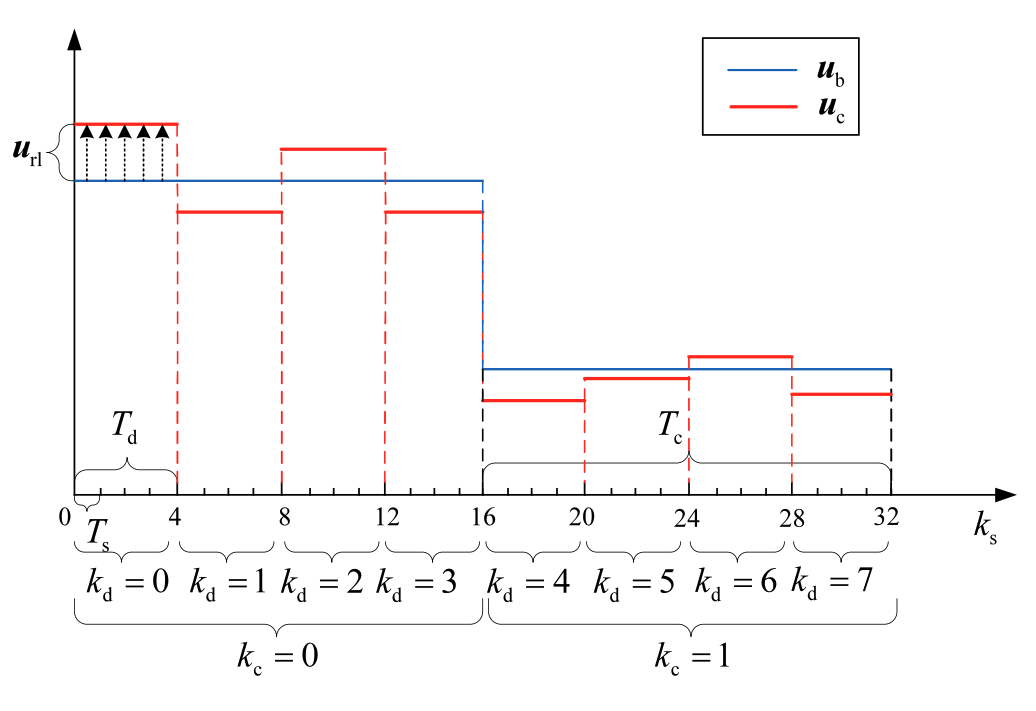
\includegraphics[width=0.8\linewidth]{figure_2.png}
    \caption{Illustration of different time scale and how DRL modifies the MPC output in the proposed hierarchical MPC-DRL framework. Taken from Sun et al.~(2024)~\cite{sun2024novel}.}
    \label{fig:framework}
\end{figure}

At the higher level, an efficient MPC component operates at a lower control frequency (e.g., every 300 seconds). Utilizing the METANET macroscopic traffic flow model, the MPC computes a baseline optimal control input over a receding prediction horizon, explicitly incorporating state and input constraints to guarantee a safe fundamental control policy. 


At the lower level, a DRL agent operates at a higher frequency (e.g., every 60 seconds) to apply online modifications to the MPC baseline output. The DRL module employs a Deep Deterministic Policy Gradient (DDPG) algorithm augmented with an $n$-step Temporal Difference (TD) method. By matching the look-ahead time of the DRL agent to the prediction horizon of the MPC module, the framework effectively compensates for model mismatches and real-time demand uncertainties. 

The original study evaluated this framework on a benchmark freeway network, comparing its performance against a no-control baseline, standalone MPC, standalone DRL, and Parameterized MPC (PMPC) across varying levels of stochastic demand noise. The authors concluded that the hierarchical approach successfully leverages the safety of MPC and the adaptability of DRL, resulting in superior reduction of Total Time Spent (TTS) and stricter constraint adherence.
\section{Implementation Details}

In this section, we detail the process of reconstructing the experiments from the original study. As no original source code was provided by the authors, all components including the traffic simulation environment, the benchmark controllers, and the hierarchical learning framework were implemented from scratch in Python.

\subsection{Building the Simulation Environment}

The original study utilizes the METANET macroscopic traffic flow model to simulate freeway dynamics. To reconstruct this environment, we leveraged the \texttt{sym\_metanet} Python library, which provides tools for the symbolic representation and simulation of macroscopic traffic networks. 

The topology of the benchmark freeway network, illustrated in Figure~\ref{fig:benchmark_network}, consists of a mainstream stretch divided into 6 segments. It includes an actively controlled on-ramp equipped with Ramp Metering (RM) and mainstream segments 3,4 equipped with Variable Speed Limits (VSL) to regulate the traffic flow proactively.

% [INSERISCI QUI L'IMMAGINE: Assicurati di caricare il file su Overleaf e cambia il nome del file in \includegraphics]
\begin{figure}[htbp]
    \centering
    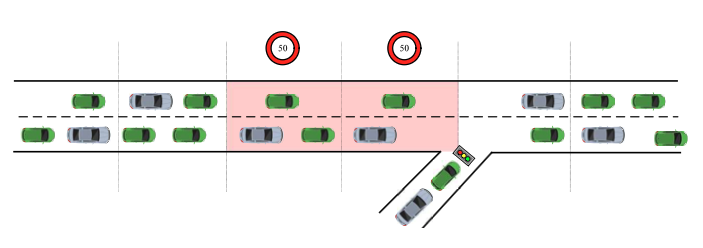
\includegraphics[width=0.8\linewidth]{figure_3.png}
    \caption{Topology of the benchmark freeway network indicating the placement of Ramp Metering (RM) and Variable Speed Limits (VSL). Taken from Sun et al.~(2024)~\cite{sun2024novel}.}
    \label{fig:benchmark_network}
\end{figure}

A primary challenge in this replication was the independent creation of the macroscopic simulation environment, as there is currently no standardized, open-source benchmark environment available for METANET. While the theoretical equations of the macroscopic model are standard, constructing an environment from scratch that accurately reproduces the macroscopic demand responses and congestion patterns of the original study proved to be a complex task. 

To address this, the calibration of our custom METANET environment was performed by systematically tuning the system to match the traffic dynamics of the original ``no-control'' scenario. Fortunately, the original manuscript provided detailed implementation specifications in their Table~III. This included explicit values for both the ``real'' system parameters utilized in the underlying simulation and the ``estimated'' model parameters used internally by the MPC controller. Leveraging these parameters significantly aided in aligning our baseline traffic dynamics with those reported by Sun et al.~(2024).

For the traffic demand generation, we exactly reproduced the deterministic demand profiles and their associated stochasticity. Following the original methodology, demand uncertainty was modeled by applying noise sampled from a Gaussian distribution (low noise $\mathcal{N}(0,75)$ for the mainline and $\mathcal{N}(0,30)$ for the ramp; medium noise $\mathcal{N}(0,150)$ for the mainline and $\mathcal{N}(0,60)$ for the ramp; high noise $\mathcal{N}(0,225)$ for the mainline and $\mathcal{N}(0,90)$ for the on-ramp demand). We evaluated the controllers across the six distinct scenarios defined in the original study, which represent varying configurations and magnitudes of demand noise. Finally, to rigorously account for the stochastic nature of both the Gaussian traffic demand and the deep reinforcement learning initialization, the final evaluation for each of the six scenarios was executed across 10 independent random seeds.



\subsection{Building the Benchmark Controllers}

To systematically evaluate the performance of the proposed hierarchical framework, we implemented the original benchmark controllers from scratch. Before detailing the control architectures, it is crucial to specify the traffic demand conditions under which they were tested.

The controllers were evaluated under a synthetic peak-hour traffic demand profile specifically designed to induce mainstream congestion and on-ramp queuing. The deterministic baseline demand consists of a mainstream inflow and an on-ramp demand that dynamically vary over the simulation period. This profile typically follows a trapezoidal pattern to accurately simulate the onset, peak duration, and subsequent dissipation of rush-hour traffic. To evaluate the robustness of the control strategies against real-world uncertainties, stochasticity was introduced to this baseline profile by adding noise sampled from a Gaussian distribution, ultimately forming the six distinct noise scenarios used in our testing phase.

\begin{figure}[htbp]
    \centering
    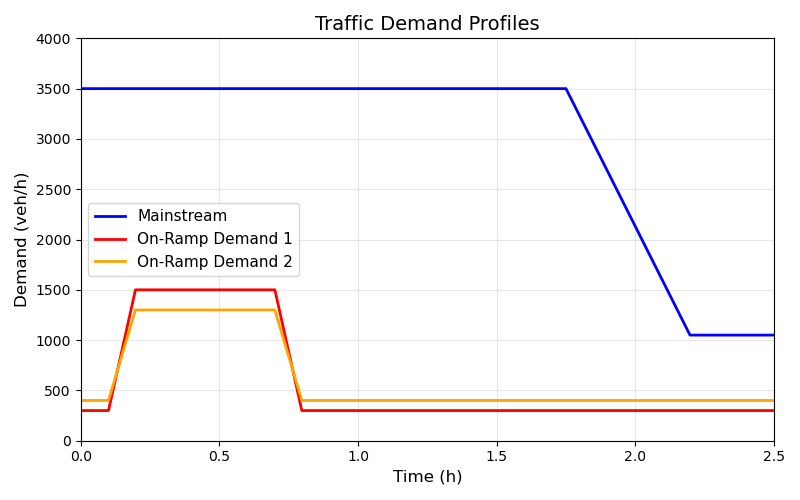
\includegraphics[width=0.8\linewidth]{figure_4.png}
    \caption{Predicted traffic demands used in the case study. Replicated from Sun et al.~(2024)~\cite{sun2024novel}.}
    \label{fig:demand_profile}
\end{figure}

Against this demand profile, the following baseline strategies were implemented to serve as benchmarks:

\begin{itemize}
    \item \textbf{No-Control Baseline:} In this configuration, no active traffic management measures are applied. The ramp metering (RM) rate is constantly maintained at its maximum allowing free flow from the ramp, and the variable speed limits (VSL) are fixed to the standard free-flow speed of the mainstream. This scenario provides the upper-bound Total Time Spent (TTS) against which the efficiency of all active controllers is measured.
    
    \item \textbf{ALINEA Controller:} As a representative of traditional, industry-standard ramp metering strategies, we implemented the ALINEA (Asservissement Linéaire d'Entrée Autoroutière) algorithm. ALINEA operates as a local, closed-loop feedback controller that dynamically adjusts the ramp metering rate based on the error between the real-time measured downstream traffic density and a predefined critical density setpoint. \textbf{It is important to underline that the ALINEA controller only meters the on-ramp, while for the VSL it only uses the free-flow speed.} In our evaluation, it serves as a robust, non-predictive baseline to benchmark the relative efficiency and constraint-handling capabilities of the advanced MPC and DRL frameworks.

    \item \textbf{Standalone MPC:} We implemented the traditional Model Predictive Control strategy using Python-based non-linear optimization tools. The standalone MPC operates at a low control frequency (e.g., a control step of 300 seconds) and solves a constrained optimization problem over a predefined prediction horizon. It leverages the ``estimated'' METANET model parameters to compute optimal RM and VSL signals that minimize TTS while strictly enforcing critical state and input constraints, such as queue length limitations and speed bound variations.
    
    \item \textbf{Standalone DRL (DDPG):} A standalone Deep Deterministic Policy Gradient (DDPG) agent was constructed. Unlike the MPC, the DRL agent operates at a high control frequency (e.g., every 60 seconds) to provide real-time continuous control actions. The actor and critic neural networks, the experience replay buffer, and the exploration noise mechanisms were implemented strictly adhering to the network architectures and hyperparameters detailed in the original manuscript.
\end{itemize}

As established in our replication scope, the Parameterized MPC (PMPC) baseline evaluated in the original study was excluded from our reconstructed benchmarks due to insufficient implementation and parameterization details in the source text. To compensate for this exclusion and provide a robust point of reference, we introduced the ALINEA controller into our evaluation suite. ALINEA was selected to test the proposed hierarchical algorithm against a well-known, state-of-the-art traditional ramp metering strategy. This addition allows us to effectively compare the performance and understand the inherent trade-offs between classical feedback control and advanced predictive or learning-based methods.

\subsection{Building the Hierarchical MPC-DRL Framework}

The core contribution of the original study is the integration of the model-based MPC and the learning-based DDPG algorithm into a cohesive, hierarchical control architecture. The fundamental principle is to operate the two controllers at different temporal resolutions: the MPC operates at a lower frequency (macro-step $T_m$) to calculate a safe, predictive baseline, while the DRL agent operates at a higher frequency (micro-step $T_c$) to apply real-time modifications.

To formalize the learning process, the high-frequency control problem is cast as a continuous Markov Decision Process (MDP) defined by the tuple $\langle \mathcal{S}, \mathcal{A}, \mathcal{P}, \mathcal{R}, \gamma \rangle$. We implemented the following formulations for the state, action, and reward spaces from scratch.

\subsubsection*{State Space Formulation}
The state $s_k \in \mathcal{S}$ at DRL control step $k$ must provide the agent with complete awareness of the current traffic conditions, the exogenous demand, and the baseline optimal intent of the high-level MPC. The state vector is formally constructed as:
\begin{equation}
    s_k = \left[ \bm{\rho}_k^T, \bm{v}_k^T, w_k, \bm{d}_k^T, (\bm{u}_{k}^{mpc})^T \right]^T
\end{equation}
where $\bm{\rho}_k$ and $\bm{v}_k$ represent the vectors of traffic densities and mainstream speeds for all segments in the METANET model, respectively; $w_k$ denotes the current queue length at the on-ramp; $\bm{d}_k$ represents the real-time measured traffic demand; and $\bm{u}_{k}^{mpc}$ is the baseline control signal (Ramp Metering and Variable Speed Limits) currently prescribed by the high-level MPC.

\subsubsection*{Action Space Formulation}
Unlike standard DRL implementations that directly output the traffic control signals, the hierarchical framework utilizes the actor network $\mu(s_k | \theta^\mu)$ to output a continuous bounded residual action $a_k \in \mathcal{A}$. 
The raw action output is defined as $a_k = [\Delta r_k, \Delta v_{c,k}]^T \in [-1, 1]^{\dim(\mathcal{A})}$, which is then denormalized to the physical bounds of the control variations.

To strictly guarantee safety and operational viability, the final control action applied to the physical environment, $u_k$, is computed by superimposing the DRL modification onto the MPC baseline, followed by a saturation function $\text{sat}_{\mathcal{U}}(\cdot)$ that saturates the signal within the strict physical constraints $\mathcal{U} = [u_{\min}, u_{\max}]$:
\begin{equation}
    u_k = \max \left( u_{\min}, \min \left( u_{\max}, u_k^{mpc} + \Delta u_k \right) \right)
\end{equation}
This clamping mechanism ensures that despite the exploratory nature of the DRL agent, the applied Variable Speed Limits and Ramp Metering rates never violate regulatory limits or induce hazardous speed drops.

\subsubsection*{Reward Formulation}
The objective of the traffic controller is to minimize the Total Time Spent (TTS) while penalizing constraint violations (such as queue overflow and drastic speed variations). The immediate reward function $r_k = \mathcal{R}(s_k, a_k)$ is formulated as the negative of the weighted system cost:
\begin{equation}
    r_k = - \left( \alpha \cdot \text{TTS}_k + \beta \cdot \Gamma_k^{queue} + \eta \cdot \Gamma_k^{speed} \right)
\end{equation}
where the instantaneous TTS is calculated based on the macroscopic METANET states:
\begin{equation}
    \text{TTS}_k = T_c \sum_{i \in \mathcal{I}} \left( \rho_{i,k} L_i \lambda_i \right) + T_c \cdot w_k
\end{equation}
Here, $L_i$ and $\lambda_i$ represent the length and the number of lanes of segment $i$, respectively. The penalty terms $\Gamma_k^{queue}$ and $\Gamma_k^{speed}$ trigger large negative values if the on-ramp queue exceeds its maximum capacity or if the temporal variation in VSL exceeds the permissible safety threshold, while $\alpha, \beta, \eta$ are positive tuning weights.

\subsubsection*{$n$-step Temporal Difference Learning Integration}
To effectively synchronize the DDPG agent with the MPC, the authors utilize an $n$-step Temporal Difference (TD) learning mechanism. Instead of relying on a standard 1-step Bellman update, the look-ahead steps $n$ of the DRL agent are explicitly matched to the prediction horizon $N_p$ of the MPC ($n \times T_c = N_p \times T_m$). 

We implemented this by modifying the DDPG replay buffer to store $n$-step transitions. The critic network $Q(s, a | \theta^Q)$ is trained to minimize the loss $\mathcal{L}(\theta^Q) = \mathbb{E} [(y_k - Q(s_k, a_k | \theta^Q))^2]$, where the target value $y_k$ incorporates the accumulated rewards over the $n$-step horizon:
\begin{equation}
    y_k = \sum_{i=0}^{n-1} \gamma^i r_{k+i} + \gamma^n Q'\left(s_{k+n}, \mu'(s_{k+n} | \theta^{\mu'}) \Big| \theta^{Q'}\right)
\end{equation}
where $\gamma \in (0, 1)$ is the discount factor, and $Q'$ and $\mu'$ denote the slowly tracking target networks. This $n$-step integration allows the learning agent to properly evaluate the delayed consequences of its actions over the exact time window optimized by the MPC, successfully bridging the model-free and model-based approaches.

\section{Results and Discussion}

In this section, we present the evaluation of the replicated hierarchical MPC-DRL framework. We compare its performance against the baseline controllers across the predefined stochastic demand scenarios. We first analyze the training dynamics of the learning algorithms, followed by a detailed assessment of their operational performance in terms of traffic efficiency and constraint satisfaction.

\newpage

\subsection{Convergence of the Learning Process}

The original study by Sun et al.~(2024) \cite{sun2024novel} reported smooth and stable convergence for the MPC-DRL agent, particularly highlighting the benefits of the $n$-step Temporal Difference (TD) learning mechanism in accelerating the training process. 

\begin{figure}[htbp]
    \centering
    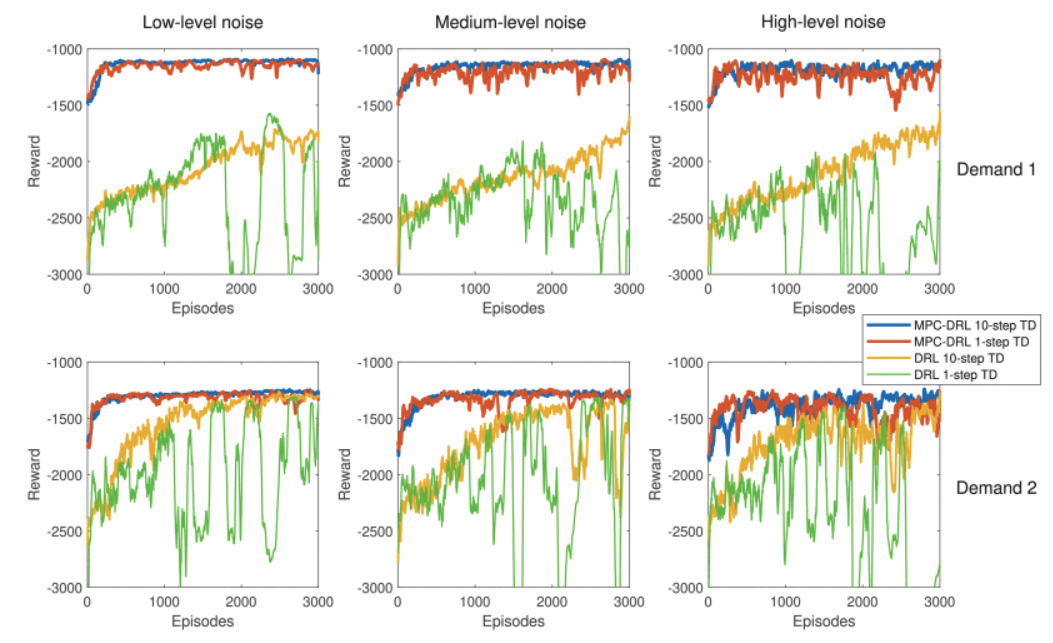
\includegraphics[width=\linewidth]{original_combined_learning_curves.png}
    \caption{Author's Learning performance of standalone DRL and combined MPC-DRL with and without 10-Step TD for different scenario. Taken from Sun et al. (2024) \cite{sun2024novel}}
    \label{fig:original_learning_curves}
\end{figure}

However, our replication efforts yielded noticeably less optimistic training dynamics.





As illustrated in Figure~\ref{fig:learning_curves}, the learning curves of the reproduced MPC-DRL framework exhibit significant instability and high variance across episodes, failing to converge to a smooth and stable plateau within the designated training timeframe.

In contrast to the claims of the original study, our results reveal markedly different learning behaviors between the standalone DRL and the hierarchical MPC-DRL framework. Specifically, the standalone DRL algorithm displays a relatively smooth learning curve, converging faster and more reliably than suggested in the original paper.

Conversely, the hierarchical MPC-DRL framework fails to achieve stable convergence. Moreover, although the overall training time is substantial for both approaches, it is disproportionately higher for the hierarchical framework. This is primarily due to the need to solve a computationally intensive constrained MPC optimization problem at every control step during the simulated training rollouts.

We attribute the observed instability in the MPC-DRL training process to several converging factors:
\begin{itemize}
    \item \textbf{Variance and Bias in $n$-step TD:} The $n$-step TD return effectively aligns the DRL look-ahead with the MPC prediction horizon. While this successfully aids eventual convergence through significant bias reduction, it intrinsically introduces higher variance to the target value $y_k$. In a noisy environment, accumulating rewards over $n$ steps aggregates the stochastic noise, causing erratic gradient updates for the Critic network.
    \item \textbf{Coupled High-Variance Stochasticity:} The Gaussian noise applied to the traffic demand creates a highly stochastic state-transition dynamic. While pure DRL handles this well, learning a residual deterministic policy on top of a dynamic MPC baseline introduces complex, non-stationary behaviors that the DDPG agent struggles to quickly stabilize.
    \item \textbf{Hyperparameter Brittleness:} The DDPG algorithm is notoriously sensitive to initialization seeds and subtle hyperparameters (e.g., exploration noise decay rates, soft update factor $\tau$). The smooth convergence of the hierarchical framework reported in the original paper may rely on highly specific, unreported initialization conditions or gradient clipping mechanisms.
    \item \textbf{Computational Bottlenecks Limiting Exploration:} Given the extreme computational cost of solving the MPC at every step during training, running an exhaustive number of training episodes is practically prohibitive. Consequently, the agent may not have sufficient episodes to adequately explore the state space and fully stabilize its residual policy before the exploration noise decays.
\end{itemize}


% [INSERISCI QUI L'IMMAGINE DELLE TUE LEARNING CURVES]
\begin{figure}[htbp]
    \centering
    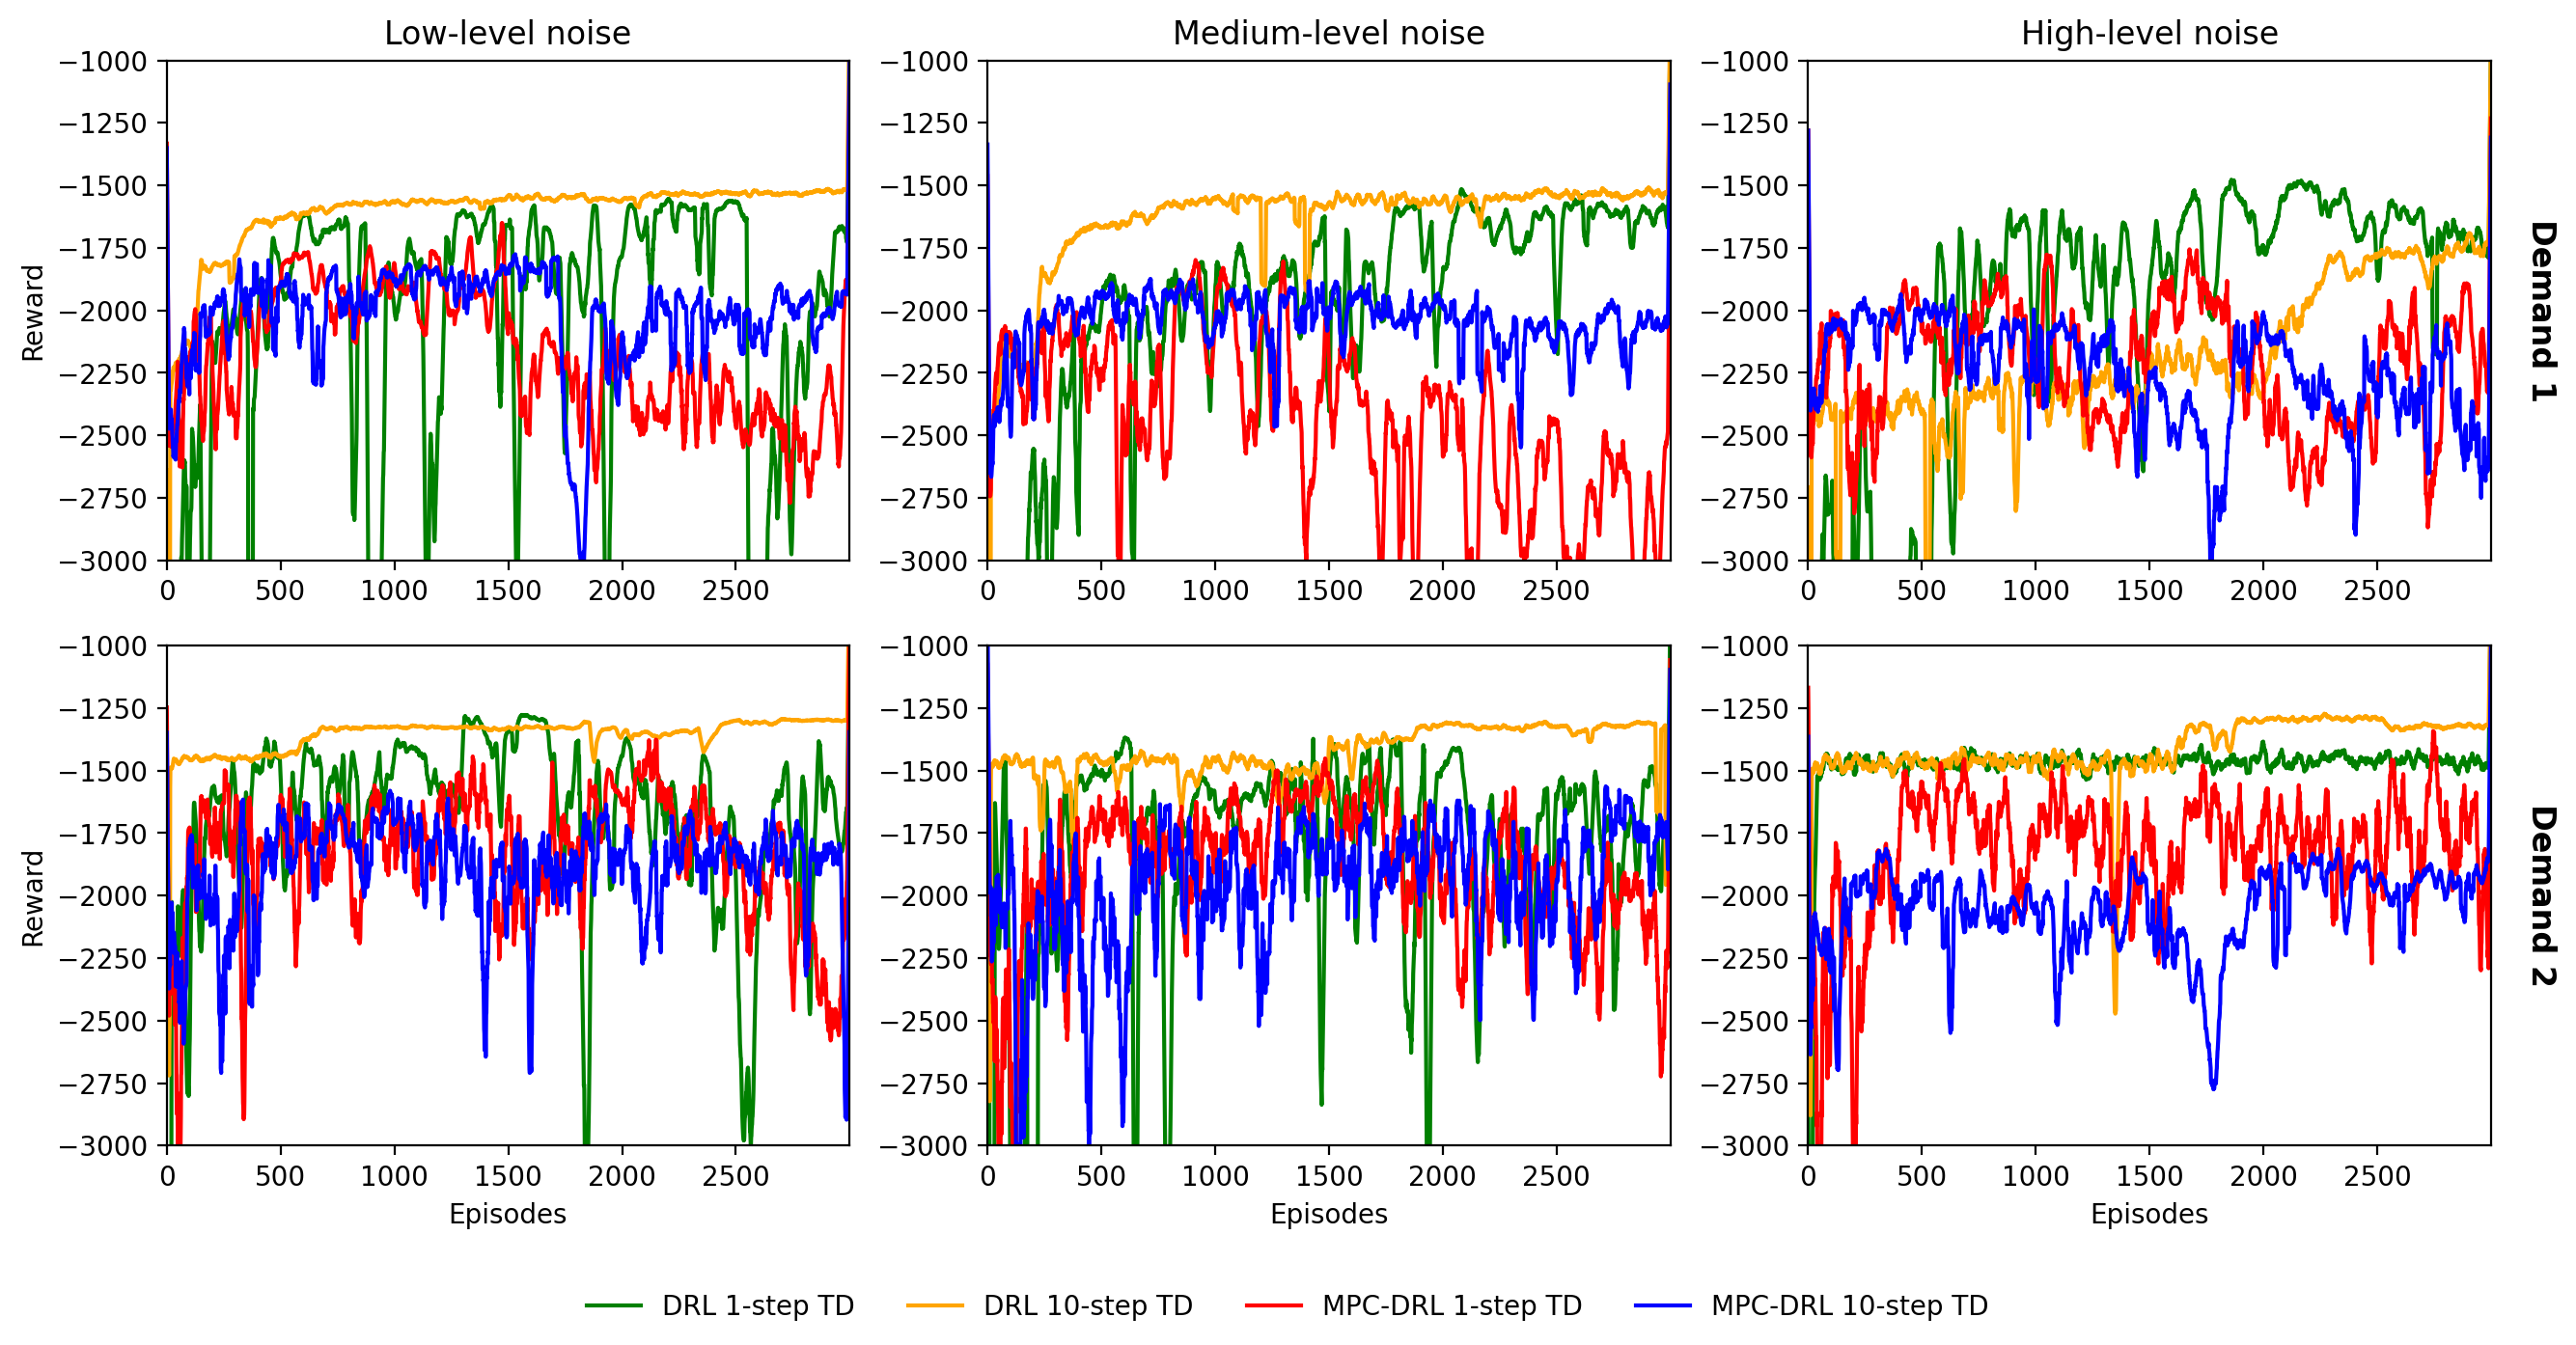
\includegraphics[width=\linewidth]{combined_learning_curves.png}
    \caption{Replicated Learning performance of standalone DRL and combined MPC-DRL with and without 10-Step TD for different scenario. Replicated from Sun et al. (2024) \cite{sun2024novel}}
    \label{fig:learning_curves}
\end{figure}


\subsection{Training Time}

Despite these training instabilities within the hierarchical framework, we successfully extracted the best-performing policy checkpoints (as well as the final policies) to evaluate their operational performance against the baselines, as discussed in the following section.

In addition to the convergence dynamics, it is crucial to analyze the sheer computational burden introduced by the hierarchical architecture during the learning phase. To ensure absolute transparency and facilitate future reproducibility efforts, we recorded the total training times for all controllers across 3000 episodes. All experiments were consistently executed on a workstation equipped with an Intel Core i7-6700 CPU @ 3.40 GHz and 32 GB of RAM.

As summarized in Table~\ref{tab:training_times}, the integration of the Model Predictive Control component strictly dominates the training duration. 

\begin{table}[htbp]
\centering
\caption{Total training time required for 3000 episodes across 6 different demand profiles, and noise levels (format: hh:mm:ss). Experiments were conducted on an Intel Core i7-6700 CPU (3.40 GHz) with 32 GB RAM.}
\label{tab:training_times}
\resizebox{\textwidth}{!}{%
\begin{tabular}{llccc}
\toprule
\textbf{Algorithm Architecture} & \textbf{Demand Profile} & \textbf{Low Noise} & \textbf{Medium Noise} & \textbf{High Noise} \\
\midrule
\multirow{2}{*}{\textbf{Standalone DRL (1-step TD)}} 
& Demand 1 & 06:18:41 & 06:15:41 & 06:41:58 \\
& Demand 2 & 09:23:02 & 09:20:11 & 09:33:07 \\
\midrule
\multirow{2}{*}{\textbf{Standalone DRL (10-step TD)}} 
& Demand 1 & 10:03:10 & 10:00:47 & 10:11:16 \\
& Demand 2 & 11:11:47 & 10:58:26 & 11:02:12 \\
\midrule
\multirow{2}{*}{\textbf{MPC-DRL Framework (1-step TD)}} 
& Demand 1 & 15:36:42 & 21:32:24 & 18:36:41 \\
& Demand 2 & 17:45:10 & 23:15:20 & 21:05:30 \\
\midrule
\multirow{2}{*}{\textbf{MPC-DRL Framework (10-step TD)}} 
& Demand 1 & 18:17:21 & 17:53:03 & 18:10:45 \\
& Demand 2 & 18:24:33 & 20:59:05 & 22:30:50 \\
\bottomrule
\end{tabular}%
}
\end{table}

The empirical data highlights a massive discrepancy between pure reinforcement learning and the hierarchical setup. While the standalone DRL agent using a standard 1-step TD update completes the training phase in roughly 6 to 9 hours (depending on the demand scenario), the hierarchical MPC-DRL framework demands significantly more computational effort, often exceeding 18 to 22 hours for the same number of episodes. 

This drastic increase in training time is fundamentally due to the fact that the computationally intensive MPC optimization problem must be formulated and solved at every single control step during the simulated training rollouts to provide the baseline action for the DRL agent. Furthermore, the inclusion of the $n$-step Temporal Difference (10-step TD) structurally increases the time required for the replay buffer transitions and Bellman updates across all architectures, further compounding the overall computational bottleneck of the training pipeline.

\subsection{Control Performance Evaluation}

To rigorously evaluate the control strategies, we extracted the best-performing policy for each scenario and executed 10 independent evaluation runs to account for the stochasticity of the Gaussian demand noise. Table~\ref{tab:results_scenario1} presents the statistical summary of these runs. To determine the statistical significance of the results, we performed a two-sample independent Student's t-test. The reported $p$-values indicate the probability that the difference between a specific baseline and the proposed hierarchical MPC-DRL framework is due to random chance (with $p < 0.05$ considered statistically significant).

\begin{table}[htbp]
\centering
\scriptsize
\setlength{\tabcolsep}{2pt}
\renewcommand{\arraystretch}{1.1}
\caption{Statistical summary (mean $\pm$ std) across 10 random seeds for all scenarios. Reported $p$-values compare each baseline against the MPC-DRL framework.}
\label{tab:results_scenario1}
\resizebox{\textwidth}{!}{%
\begin{tabular}{llcccccc}
\toprule
Scenarios & Performance & No control & Standalone ALINEA & Standalone MPC & Standalone DRL & HF MPC & MPC-DRL framework \\
\midrule
Scenario 1 & Total time spent [veh·h] & 1428.40 $\pm$ 9.04 (p=0.000) & 1188.92 $\pm$ 8.05 (p=0.000) & 1428.89 $\pm$ 9.07 (p=0.000) & 1377.41 $\pm$ 9.47 (p=0.000) & 1398.58 $\pm$ 8.90 (p=0.050) & 1405.26 $\pm$ 14.94 \\
 & Total waiting time [veh·h] & 340.96 $\pm$ 6.50 (p=0.001) & 394.57 $\pm$ 5.91 (p=0.000) & 341.84 $\pm$ 6.53 (p=0.001) & 321.99 $\pm$ 6.59 (p=0.000) & 317.54 $\pm$ 6.39 (p=0.000) & 350.90 $\pm$ 10.20 \\
 & Minimum speed [km/h] & 12.63 $\pm$ 0.06 (p=0.000) & 31.10 $\pm$ 0.72 (p=0.000) & 12.46 $\pm$ 0.12 (p=0.000) & 12.15 $\pm$ 0.03 (p=0.000) & 13.98 $\pm$ 0.05 (p=0.000) & 13.28 $\pm$ 0.05 \\
 & Constraint violation [\%] & 84.36 $\pm$ 2.33 (p=0.000) & 330.75 $\pm$ 5.66 (p=0.000) & 80.20 $\pm$ 2.42 (p=0.000) & 48.04 $\pm$ 3.25 (p=0.000) & 62.25 $\pm$ 2.30 (p=0.000) & 28.96 $\pm$ 1.17 \\
 & Mean computation time [s] & - & - & 10.67 $\pm$ 0.39 (p=0.000) & 0.00 $\pm$ 0.00 (p=0.000) & 55.13 $\pm$ 7.33 (p=0.000) & 0.41 $\pm$ 0.06 \\
 & Max computation time [s] & - & - & 76.14 $\pm$ 1.69 (p=0.000) & 0.00 $\pm$ 0.00 (p=0.000) & 343.49 $\pm$ 60.26 (p=0.000) & 3.27 $\pm$ 1.63 \\
\midrule
Scenario 2 & Total time spent [veh·h] & 1425.58 $\pm$ 18.06 (p=0.000) & 1185.81 $\pm$ 17.12 (p=0.000) & 1426.11 $\pm$ 18.18 (p=0.000) & 1376.23 $\pm$ 18.46 (p=0.000) & 1395.83 $\pm$ 18.59 (p=0.000) & 1419.31 $\pm$ 18.78 \\
 & Total waiting time [veh·h] & 338.30 $\pm$ 12.97 (p=0.000) & 391.53 $\pm$ 13.84 (p=0.000) & 339.22 $\pm$ 13.08 (p=0.000) & 313.61 $\pm$ 11.97 (p=0.000) & 314.95 $\pm$ 13.35 (p=0.000) & 333.83 $\pm$ 12.88 \\
 & Minimum speed [km/h] & 12.61 $\pm$ 0.11 (p=0.000) & 30.79 $\pm$ 0.89 (p=0.000) & 12.49 $\pm$ 0.17 (p=0.000) & 12.11 $\pm$ 0.05 (p=0.000) & 14.02 $\pm$ 0.14 (p=0.000) & 14.52 $\pm$ 0.10 \\
 & Constraint violation [\%] & 83.44 $\pm$ 4.61 (p=0.000) & 331.92 $\pm$ 12.02 (p=0.000) & 78.99 $\pm$ 4.83 (p=0.000) & 41.27 $\pm$ 6.66 (p=0.000) & 61.37 $\pm$ 4.80 (p=0.000) & 20.16 $\pm$ 3.09 \\
 & Mean computation time [s] & - & - & 7.85 $\pm$ 0.22 (p=0.000) & 0.00 $\pm$ 0.00 (p=0.000) & 52.15 $\pm$ 2.16 (p=0.000) & 0.45 $\pm$ 0.11 \\
 & Max computation time [s] & - & - & 57.02 $\pm$ 0.62 (p=0.000) & 0.00 $\pm$ 0.00 (p=0.001) & 328.02 $\pm$ 22.28 (p=0.000) & 3.65 $\pm$ 2.23 \\
\midrule
Scenario 3 & Total time spent [veh·h] & 1422.86 $\pm$ 27.06 (p=0.000) & 1180.55 $\pm$ 24.48 (p=0.000) & 1423.43 $\pm$ 27.17 (p=0.000) & 1415.09 $\pm$ 27.78 (p=0.006) & 1393.32 $\pm$ 27.81 (p=0.000) & 1418.24 $\pm$ 27.33 \\
 & Total waiting time [veh·h] & 335.75 $\pm$ 19.40 (p=0.630) & 387.48 $\pm$ 19.67 (p=0.000) & 336.60 $\pm$ 19.44 (p=0.035) & 339.45 $\pm$ 18.58 (p=0.001) & 312.71 $\pm$ 19.91 (p=0.000) & 335.50 $\pm$ 19.48 \\
 & Minimum speed [km/h] & 12.60 $\pm$ 0.17 (p=0.218) & 31.43 $\pm$ 1.23 (p=0.000) & 12.47 $\pm$ 0.23 (p=0.495) & 12.17 $\pm$ 0.11 (p=0.000) & 14.02 $\pm$ 0.17 (p=0.000) & 12.52 $\pm$ 0.09 \\
 & Constraint violation [\%] & 82.58 $\pm$ 6.87 (p=0.000) & 328.92 $\pm$ 11.40 (p=0.000) & 78.15 $\pm$ 6.87 (p=0.000) & 74.69 $\pm$ 15.09 (p=0.000) & 60.59 $\pm$ 7.22 (p=0.000) & 39.33 $\pm$ 6.19 \\
 & Mean computation time [s] & - & - & 7.83 $\pm$ 0.26 (p=0.000) & 0.00 $\pm$ 0.00 (p=0.000) & 49.31 $\pm$ 4.14 (p=0.000) & 0.37 $\pm$ 0.04 \\
 & Max computation time [s] & - & - & 56.84 $\pm$ 0.23 (p=0.000) & 0.00 $\pm$ 0.00 (p=0.000) & 331.59 $\pm$ 27.62 (p=0.000) & 2.04 $\pm$ 0.19 \\
\midrule
Scenario 4 & Total time spent [veh·h] & 1320.35 $\pm$ 9.67 (p=0.942) & 1089.62 $\pm$ 7.51 (p=0.000) & 1313.79 $\pm$ 14.41 (p=0.719) & 1321.85 $\pm$ 9.03 (p=0.864) & 1275.05 $\pm$ 9.97 (p=0.015) & 1319.27 $\pm$ 46.63 \\
 & Total waiting time [veh·h] & 228.70 $\pm$ 6.63 (p=0.005) & 294.08 $\pm$ 5.77 (p=0.208) & 225.48 $\pm$ 10.23 (p=0.004) & 247.66 $\pm$ 6.69 (p=0.014) & 196.75 $\pm$ 6.58 (p=0.001) & 331.02 $\pm$ 85.95 \\
 & Minimum speed [km/h] & 15.20 $\pm$ 0.05 (p=0.000) & 30.95 $\pm$ 0.84 (p=0.000) & 15.18 $\pm$ 0.39 (p=0.000) & 20.85 $\pm$ 0.02 (p=0.002) & 16.35 $\pm$ 0.33 (p=0.000) & 22.41 $\pm$ 1.15 \\
 & Constraint violation [\%] & 20.77 $\pm$ 2.48 (p=0.000) & 220.10 $\pm$ 5.44 (p=0.001) & 14.23 $\pm$ 3.51 (p=0.000) & 12.85 $\pm$ 2.09 (p=0.000) & 0.00 $\pm$ 0.00 (p=0.000) & 154.06 $\pm$ 42.69 \\
 & Mean computation time [s] & - & - & 8.64 $\pm$ 2.08 (p=0.000) & 0.00 $\pm$ 0.00 (p=0.000) & 73.36 $\pm$ 5.73 (p=0.000) & 0.67 $\pm$ 0.19 \\
 & Max computation time [s] & - & - & 62.94 $\pm$ 6.43 (p=0.000) & 0.00 $\pm$ 0.00 (p=0.000) & 467.46 $\pm$ 52.71 (p=0.000) & 7.31 $\pm$ 1.94 \\
\midrule
Scenario 5 & Total time spent [veh·h] & 1317.74 $\pm$ 19.33 (p=0.702) & 1086.45 $\pm$ 14.91 (p=0.000) & 1310.61 $\pm$ 28.66 (p=0.004) & 1306.07 $\pm$ 18.57 (p=0.001) & 1271.67 $\pm$ 20.33 (p=0.000) & 1316.93 $\pm$ 24.13 \\
 & Total waiting time [veh·h] & 226.31 $\pm$ 13.23 (p=0.645) & 291.16 $\pm$ 13.04 (p=0.000) & 222.61 $\pm$ 19.66 (p=0.001) & 213.74 $\pm$ 13.29 (p=0.000) & 194.28 $\pm$ 13.73 (p=0.000) & 227.08 $\pm$ 17.28 \\
 & Minimum speed [km/h] & 15.20 $\pm$ 0.09 (p=0.191) & 31.39 $\pm$ 0.88 (p=0.000) & 15.18 $\pm$ 0.49 (p=0.035) & 15.20 $\pm$ 0.09 (p=0.191) & 16.32 $\pm$ 0.28 (p=0.000) & 15.33 $\pm$ 0.31 \\
 & Constraint violation [\%] & 19.94 $\pm$ 4.92 (p=0.781) & 221.94 $\pm$ 8.69 (p=0.000) & 13.08 $\pm$ 5.52 (p=0.000) & 19.51 $\pm$ 9.41 (p=0.712) & 0.00 $\pm$ 0.00 (p=0.000) & 20.16 $\pm$ 6.80 \\
 & Mean computation time [s] & - & - & 11.71 $\pm$ 3.24 (p=0.000) & 0.00 $\pm$ 0.00 (p=0.000) & 68.18 $\pm$ 4.72 (p=0.000) & 0.46 $\pm$ 0.10 \\
 & Max computation time [s] & - & - & 99.30 $\pm$ 58.32 (p=0.000) & 0.00 $\pm$ 0.00 (p=0.000) & 429.08 $\pm$ 42.89 (p=0.000) & 3.52 $\pm$ 1.79 \\
\midrule
Scenario 6 & Total time spent [veh·h] & 1315.19 $\pm$ 28.97 (p=0.983) & 1083.17 $\pm$ 21.15 (p=0.000) & 1304.74 $\pm$ 38.99 (p=0.012) & 1326.01 $\pm$ 29.90 (p=0.006) & 1269.76 $\pm$ 29.95 (p=0.000) & 1315.25 $\pm$ 35.24 \\
 & Total waiting time [veh·h] & 224.01 $\pm$ 19.77 (p=0.723) & 289.01 $\pm$ 18.13 (p=0.000) & 218.05 $\pm$ 26.84 (p=0.026) & 258.11 $\pm$ 17.64 (p=0.000) & 192.42 $\pm$ 19.83 (p=0.000) & 224.78 $\pm$ 24.81 \\
 & Minimum speed [km/h] & 15.19 $\pm$ 0.13 (p=0.000) & 31.05 $\pm$ 1.18 (p=0.000) & 15.23 $\pm$ 0.68 (p=0.000) & 17.00 $\pm$ 0.34 (p=0.008) & 16.46 $\pm$ 0.36 (p=0.124) & 16.61 $\pm$ 0.22 \\
 & Constraint violation [\%] & 19.13 $\pm$ 7.36 (p=0.000) & 219.92 $\pm$ 8.74 (p=0.000) & 12.32 $\pm$ 7.06 (p=0.088) & 91.50 $\pm$ 16.37 (p=0.000) & 0.00 $\pm$ 0.00 (p=0.000) & 10.57 $\pm$ 5.58 \\
 & Mean computation time [s] & - & - & 13.01 $\pm$ 7.09 (p=0.000) & 0.00 $\pm$ 0.00 (p=0.000) & 66.56 $\pm$ 3.66 (p=0.000) & 0.46 $\pm$ 0.10 \\
 & Max computation time [s] & - & - & 101.38 $\pm$ 56.67 (p=0.000) & 0.00 $\pm$ 0.00 (p=0.000) & 411.20 $\pm$ 20.87 (p=0.000) & 3.27 $\pm$ 1.69 \\
\bottomrule
\end{tabular}%
}
\end{table}

The empirical results confirm several trends reported in the original study, while also highlighting crucial operational trade-offs. 

Firstly, the traditional ALINEA controller yields the lowest Total Time Spent (TTS) on the mainstream freeway ($1188.92$ veh·h). However, this seemingly superior performance masks a severe limitation: as a closed-loop controller focusing solely on mainstream density, ALINEA aggressively restricts the on-ramp inflow. This results in a massive queue spillback effect, demonstrated by an unacceptable constraint violation with a pick rate of $331.92\%$. While ALINEA successfully clears the highway, it simply displaces the congestion onto the unmodeled urban road network, failing to provide a holistic traffic management solution.

Secondly, the results clearly illustrate the computation-safety trade-off between the advanced controllers. The High-Frequency MPC (HF MPC) successfully achieves perfect safety (0\% constraint violations with Demand profile 2). However, its mean computation time per step is approximatly $68$ seconds. While absolute computation times are hardware-dependent, exceeding the actual $60$-second control step renders the HF MPC physically unviable for real-time deployment. Conversely, the Standalone DRL is fast and effective at minimizing TTS, but it fails to strictly respect system constraints. 

The proposed MPC-DRL framework effectively positions itself as a pragmatic compromise. It maintains a very low computation footprint (pick of $0.67$ seconds) suitable for real-time applications while delivering TTS performance comparable to the learning-based baselines. It should be noted, however, that in this specific evaluation, the hierarchical framework did not completely eliminate constraint violations, suggesting that the high-frequency DRL modifications can still occasionally override the baseline safety guarantees of the low-frequency MPC.

\subsection{Discussion and Limitations}

Beyond the numerical outcomes, our replication efforts revealed two significant methodological limitations in the original study that warrant further discussion.

\textbf{Realism of the Demand Profile:} The evaluation in the original paper heavily relies on a step-like (trapezoidal) deterministic demand profile. In our experience, such abrupt, discontinuous demand functions are generally atypical for macroscopic continuous models like METANET. Real-world macroscopic traffic demand usually follows smoother, continuous distributions. The use of step functions may induce artificial shockwaves in the simulation that skew the evaluation of predictive controllers.

\textbf{Lack of Model Generalization:} The original study's methodology involves training a distinct DRL agent for each specific noise scenario. While this successfully demonstrates that the architecture can learn to optimize a specific traffic distribution, it is fundamentally misleading from a practical deployment perspective. In real-world intelligent transportation systems, training a new agent for every minor shift in demand is unfeasible. A robust, deployable reinforcement learning controller must demonstrate generalization capabilities: meaning a single, unified model trained across a wide distribution of scenarios should be able to perform adequately under varying unseen traffic conditions. We suggest that future research on this framework should pivot from scenario-specific overfitting to evaluating the zero-shot generalization of a uniformly trained MPC-DRL agent.
\newpage

\section{Conclusion}

This work set out to reproduce \textit{``A Novel Framework Combining MPC and Deep Reinforcement Learning With Application to Freeway Traffic Control''} from Sun et al.\ (2024), originally published in IEEE Transactions on Intelligent Transportation Systems~\cite{sun2024novel}.

Although only the information provided in the original publication was available, and no source code, simulation environment, or dataset was provided, the comprehensive methodological descriptions and hyperparameter tables allowed for a full reconstruction of the original work from scratch. During the replication, several operational trade-offs and methodological limitations were identified and systematically evaluated:

\begin{itemize}
    \item The independent construction and calibration of the METANET macroscopic environment proved highly challenging, highlighting the critical need for standardized, open-source benchmark environments in traffic flow modeling.
    \item Our replication confirmed the fundamental computational and safety trade-offs of the standalone methods: High-Frequency MPC (HF MPC) guarantees strict safety but violates real-time computational constraints, whereas pure DRL is computationally efficient but fails to reliably respect system constraints.
    \item The reproduced MPC-DRL framework successfully demonstrated its value as a highly effective compromise. By extracting the high-speed computational inference from the DRL agent and anchoring it to the safety bounds of the low-frequency MPC, it bridges the gap between theoretical optimality and practical real-time application.
    \item However, the training process exhibited significant instability under stochastic demand, diverging from the smooth convergence reported originally.
\end{itemize}

Despite its strong theoretical appeal and successful replication, our findings suggest that the proposed hierarchical framework is not unilaterally the ``best'' method for all scenarios. Depending on the specific traffic management goals, traditional or standalone controllers might still be preferable. For instance, if the sole objective is to maximize mainstream throughput regardless of ramp queuing, ALINEA performs exceptionally well with a fraction of the implementation complexity. 

Furthermore, the current framework relies on scenario-specific training, which severely limits its out-of-the-box applicability. We highlight that while the architecture is robust, future work must focus on the model's generalization capabilities, training a unified agent capable of adapting to diverse, unseen traffic distributions without requiring scenario-specific retraining.

Nonetheless, this reproduction resulted in a fully functional, open-source Python repository encompassing the simulation environment, traditional benchmark controllers, and the complete hierarchical reinforcement learning training pipeline. This work contributes to the broader mission of advancing reproducible research practices in intelligent transportation systems by promoting open science principles, developing transparent baselines, and fostering community engagement.

\newpage